

I implemented the blocked \href{./../src/3-Optimize-Matrix-Matrix-Mult/dgemm-blocked.c}{DGEMM} as prescribed in the assignment and processed it on the cluster with different block sizes; the plots in Figure~\ref{fig:dgemm-performance} collect the timing traces.

I produced \href{./../src/3-Optimize-Matrix-Matrix-Mult/dgemm-blocked-omp.c}{dgemm-blocked-omp.c} implementing the requested OpenMP parallelism, compiler flags, and the same block-size sweep to compare the tuned path. Unfortunately, the OpenMP version \textbf{did not} outperform the baseline in any configuration and I'm not sure why.

\begin{figure}[H]
    \centering
    \begin{subfigure}[b]{0.48\textwidth}
        \centering
        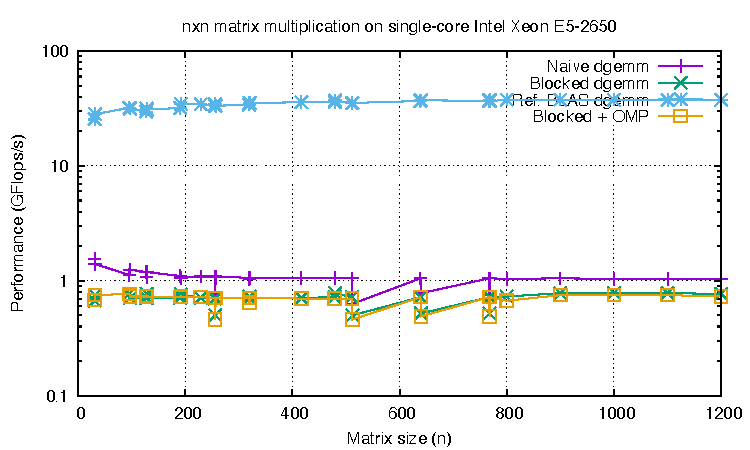
\includegraphics[width=\textwidth]{../src/3-Optimize-Matrix-Matrix-Mult/results/timing-02.pdf}
        \caption{Block size = 2}
        \label{fig:timing-02}
    \end{subfigure}
    \hfill
    \begin{subfigure}[b]{0.48\textwidth}
        \centering
        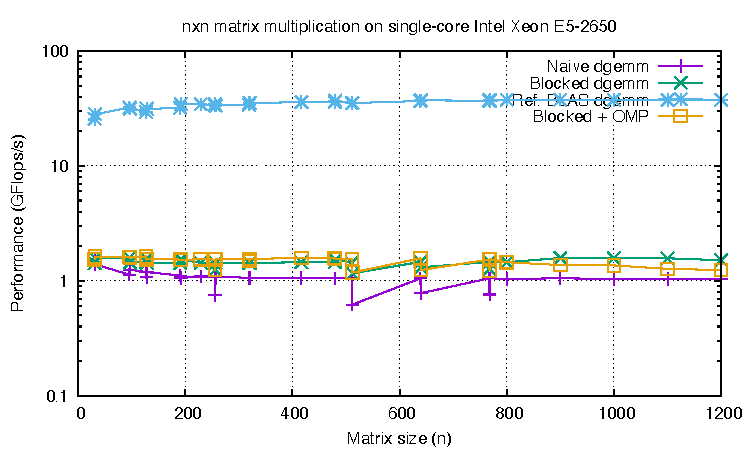
\includegraphics[width=\textwidth]{../src/3-Optimize-Matrix-Matrix-Mult/results/timing-04.pdf}
        \caption{Block size = 4}
        \label{fig:timing-04}
    \end{subfigure}
    
    \vspace{1em}
    
    \begin{subfigure}[b]{0.48\textwidth}
        \centering
        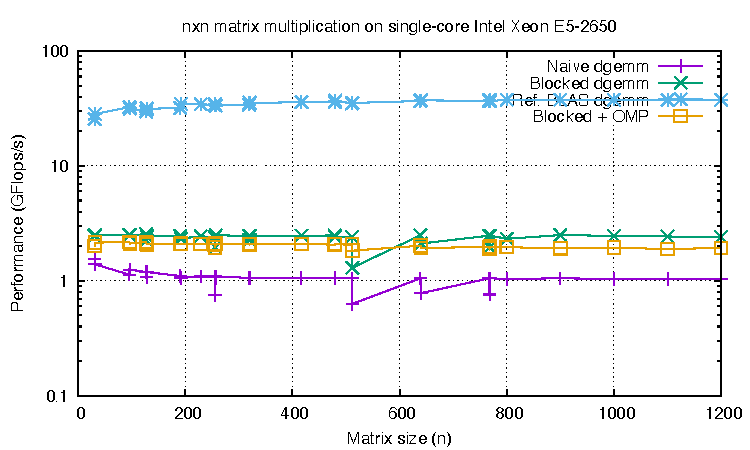
\includegraphics[width=\textwidth]{../src/3-Optimize-Matrix-Matrix-Mult/results/timing-08.pdf}
        \caption{Block size = 8}
        \label{fig:timing-08}
    \end{subfigure}
    \hfill
    \begin{subfigure}[b]{0.48\textwidth}
        \centering
        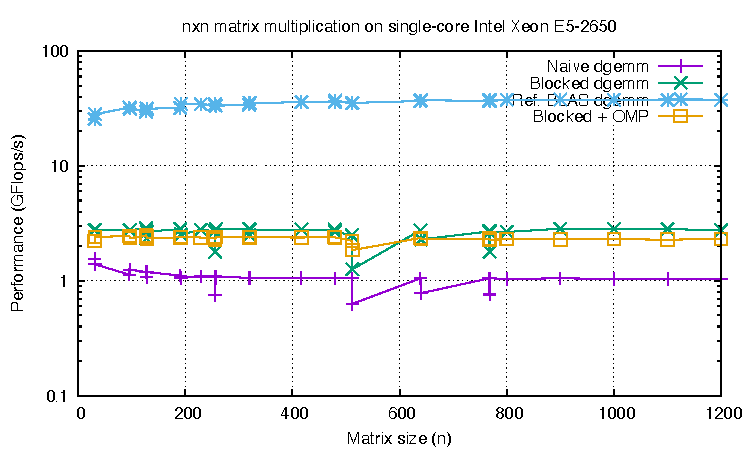
\includegraphics[width=\textwidth]{../src/3-Optimize-Matrix-Matrix-Mult/results/timing-16.pdf}
        \caption{Block size = 16}
        \label{fig:timing-16}
    \end{subfigure}
    
    \vspace{1em}
    
    \begin{subfigure}[b]{0.48\textwidth}
        \centering
        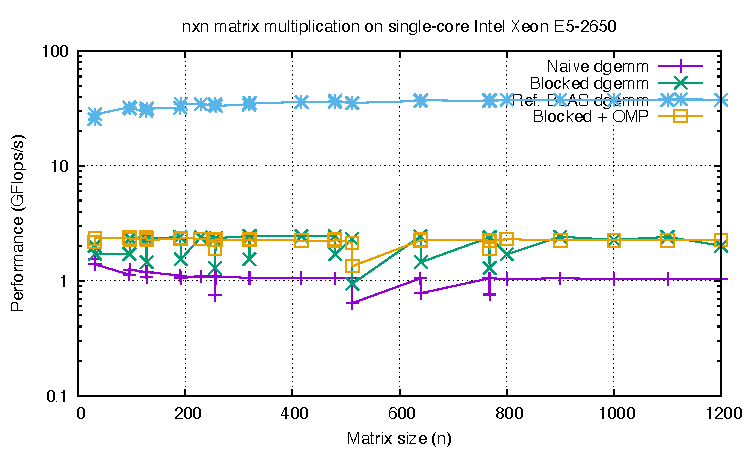
\includegraphics[width=\textwidth]{../src/3-Optimize-Matrix-Matrix-Mult/results/timing-32.pdf}
        \caption{Block size = 32}
        \label{fig:timing-32}
    \end{subfigure}
    \hfill
    \begin{subfigure}[b]{0.48\textwidth}
        \centering
        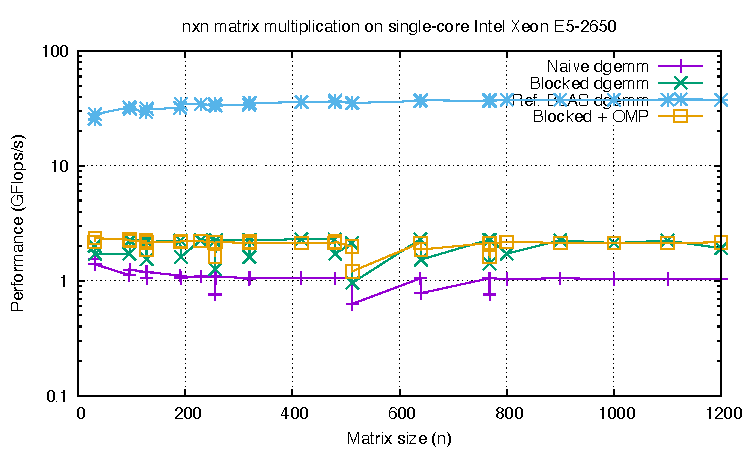
\includegraphics[width=\textwidth]{../src/3-Optimize-Matrix-Matrix-Mult/results/timing-64.pdf}
        \caption{Block size = 64}
        \label{fig:timing-64}
    \end{subfigure}
    
    \caption{Performance comparison of different DGEMM implementations with different block sizes}
    \label{fig:dgemm-performance}
\end{figure}

I summarized each run from the \texttt{matrixmult-*.out} logs in \href{./../src/3-Optimize-Matrix-Matrix-Mult/results}{results/} and reported them in Table~\ref{tab:performance-summary}. This includes the averages for each model and each block size. The rough binary search still points to block size 16 as the best baseline (7.06\% of peak). A more refined search could still reveal a stronger configuration.

\begin{table}[H]
\centering
\begin{tabular}{|l|c|c|c|}
\hline
\textbf{Implementation} & \textbf{Block Size} & \textbf{Blocked Avg. \%} & \textbf{Blocked + OMP Avg. \%} \\
\hline
\hline
Naive DGEMM & -- & 2.88\% & -- \\
\hline
BLAS DGEMM & -- & 93.77\% & -- \\
\hline
\hline
\multirow{6}{*}{Blocked DGEMM} 
& 2  & 1.91\% & 1.87\% \\
\cline{2-4}
& 4  & 3.94\% & 4.01\% \\
\cline{2-4}
& 8  & 6.41\% & 5.53\% \\
\cline{2-4}
& 16 & 7.06\% & 6.35\% \\
\cline{2-4}
& 32 & 5.55\% & 6.04\% \\
\cline{2-4}
& 64 & 5.36\% & 5.66\% \\
\hline
\end{tabular}
\caption{Average Percentage of Peak Performance}
\label{tab:performance-summary}
\end{table}

The tuned OpenMP path gives the higher block sizes a lift (for example +0.5 points at block size 32), so it is the version I would keep scaling even if the single-node sweet spot stays around block size 16.
